% !TEX program = lualatex
\documentclass[12pt,a4paper]{article}
\usepackage{graphicx}
\usepackage{fontspec}
\setmonofont{Latin Modern Mono}
\usepackage{xcolor}
\usepackage{listings}
\usepackage{geometry}
\usepackage{fancyhdr}
\usepackage{hyperref}
\usepackage{booktabs} 
\usepackage{float}    
\usepackage{amsmath}

% =======================================================
%  USER CONFIGURATION
% =======================================================
\newcommand{\labNo}{Lab 6}
\newcommand{\labTopic}{Operation Shadow Protocol: Views, Roles, String, Sets \& Dates}
\newcommand{\courseCode}{CSE 4308}
\newcommand{\courseTitleShort}{DBMS Lab}
\newcommand{\courseTitleLong}{DATABASE MANAGEMENT SYSTEMS LAB}
\newcommand{\instructorName}{Samnun Azfar, Jr. Lecturer, CSE\\ Samia Nawsheen, Jr. Lecturer, CSE}
\newcommand{\academicYear}{AY25-26}
% =======================================================

\geometry{margin=1in}

% -
% Header and Footer Configuration
% -
\pagestyle{fancy}
\fancyhf{}
\lhead{\labNo}                        
\rhead{\courseCode: \courseTitleShort} 

\cfoot{\thepage}
\setlength{\headwidth}{\textwidth}

% -
% Code Listing Style
% -
\definecolor{codegreen}{rgb}{0,0.6,0}
\definecolor{codegray}{rgb}{0.5,0.5,0.5}
\definecolor{codepurple}{rgb}{0.58,0,0.82}
\definecolor{backcolour}{rgb}{0.95,0.95,0.92}

\lstdefinestyle{mystyle}{
    backgroundcolor=\color{backcolour},
    commentstyle=\color{codegreen},
    keywordstyle=\color{magenta},
    numberstyle=\tiny\color{codegray},
    stringstyle=\color{codepurple},
    basicstyle=\ttfamily\footnotesize,
    breaklines=true,
    captionpos=b,
    keepspaces=true,
    numbers=left,
    numbersep=5pt,
    tabsize=2,
    frame=single,
    numbers=none,
    columns=fullflexible,
    showspaces=false,
    showstringspaces=false,
    showtabs=false,
    language=SQL
}

\lstset{style=mystyle}

% Images: found next to this file (local compile_labs.sh) or via the
% lab folder when compiled from the project root (Overleaf).
\graphicspath{{lab_06_views_roles_string_sets_dates/}}

\begin{document}

% --
% TITLE PAGE
% --
\begin{titlepage}
    \centering
    \vspace*{2\baselineskip}

    \rule{14cm}{2pt}\vspace*{-0.8\baselineskip}\vspace*{1.5pt}
    \rule{14cm}{0.5pt}\vspace{2\baselineskip}

    {\Huge\bfseries\scshape \labNo\par} 
    \vspace{3mm}
    {\Large \labTopic} 
    \vspace{3mm}

    \rule{14cm}{0.5pt}\vspace*{-0.7\baselineskip}\vspace{2.5pt}
    \rule{14cm}{2pt}

    \vspace{2\baselineskip}

    {\Large\bfseries \courseCode\par} 
    \vspace{1\baselineskip}
    {\large \courseTitleLong\par} 

    \vfill
    {\normalsize Prepared by:\\ \instructorName\par} 
    {\normalsize Academic Year: \academicYear\par} 
\end{titlepage}

\newpage
\tableofcontents
\newpage
\section*{Lab Workflow}



\textit{Repeat this subsection for every single lab.}

\begin{enumerate}
\item Connect to the internet by running nmtui in terminal, add a dsl connection, then go back and activate that dsl connection. Make sure that your net id is not being used in any other pc or router, if you face any issue, use any other net id from your friends which is not being used.

\item Download all the files posted in the google classroom.

\item Disconnect from the \textbf{dsl} connection via nmtui, connect to the ethernet/wired connection via nmtui. If no such connection exists, create an \textbf{ethernet} connection  and then activate.

    \item \textbf{Create Your Role and Database}

Inside the PostgreSQL shell, create your own role (user) and database.

1. In the Linux terminal:
\begin{lstlisting}[language=bash]
psql
\end{lstlisting}

Expected prompt:
\begin{lstlisting}
cse=#
\end{lstlisting}

2. Create Your Role and Database

Copy and run the following commands inside PostgreSQL:
\begin{lstlisting}[language=SQL]
-- 1. Terminate existing database connections
SELECT pg_terminate_backend(pid)
FROM pg_stat_activity
WHERE datname = 'cse4308_12345'
  AND pid <> pg_backend_pid();

-- 2. Remove existing database
DROP DATABASE IF EXISTS cse4308_12345;

-- 3. Remove existing role
DROP ROLE IF EXISTS student_12345;

-- 4. Create role
CREATE ROLE student_12345 LOGIN;

-- 5. Set password
ALTER ROLE student_12345
WITH PASSWORD 'student12345';

-- 6. Create database
CREATE DATABASE cse4308_12345
OWNER student_12345;

-- 7. Grant privileges
GRANT ALL PRIVILEGES
ON DATABASE cse4308_12345
TO student_12345;
\end{lstlisting}

3. Exit PostgreSQL:

   \begin{lstlisting}[language=SQL]
   \q
   \end{lstlisting}

\item \textbf{Connect Using Your Newly Created User}

1. Connect to Your Database:

   Use the following command to log in as the \texttt{student\_12345} user:

   \begin{lstlisting}[language=SQL]
   psql -h localhost -U student_12345 -d cse4308_12345
   \end{lstlisting}

2. Verify the Connection:

   Verify that you are connected to the correct database with the following command:

   \begin{lstlisting}[language=SQL]
   \conninfo
   \end{lstlisting}

   Expected output:

   \begin{lstlisting}
   Database: cse4308_12345, User: student_12345
   \end{lstlisting}

3. Exit PostgreSQL:

   \begin{lstlisting}[language=SQL]
   \q
   \end{lstlisting}

\item \textbf{Load the Lab SQL File (MUST be run outside psql)}

Load the SQL file that sets up the tables and inserts initial data.

1. Load the SQL File:

   Run the following command to load the lab SQL file:

   \begin{lstlisting}[language=SQL]
   psql -h localhost -U student_12345 -d cse4308_12345 -f /home/cse/Downloads/lab_06_setup.sql
   \end{lstlisting}

   This will:
   - Drop old tables (if they exist).
   - Create new tables.
   - Insert initial rows of data.

\item \textbf{Reconnect and Verify Tables}

After loading the SQL file, reconnect to PostgreSQL to verify that the tables have been created.

1. Reconnect to Your Database:

   \begin{lstlisting}[language=SQL]
   psql -h localhost -U student_12345 -d cse4308_12345
   \end{lstlisting}

2. Check Tables:

   Verify the tables have been created by listing them:

   \begin{lstlisting}[language=SQL]
   \dt
   \end{lstlisting}

3. View Table Data:

   Verify the data by running the following SQL queries:

   \begin{lstlisting}[language=SQL]
   SELECT * FROM <table_name>;
   \end{lstlisting}

\item Open a text editor and save it in the appropriate submission name format \\ \texttt{fullid\_CSE4308\_L6\_T1.sql}. You will use this text editor to write your solutions, make sure to save it after writing each solution. The structure of this file will be:
\begin{lstlisting}[language=SQL]
-- Task 1
INSERT INTO students (student_id, name, major, gpa)
VALUES (104, 'David', 'ME', 3.60);
--Task 2
SELECT name, gpa FROM students WHERE major = 'CSE';
\end{lstlisting}
\end{enumerate}
\newpage

\section{Introduction}
This lab module demonstrates advanced data manipulation techniques in PostgreSQL. We will cover character string processing for data cleaning, temporal operations for date logic, set-theoretic operators for combining datasets, and Data Control Language (DCL) for security management.

\section{Lab Environment Setup}
Before executing the functional demonstrations, you must create the schema and populate the tables. Execute the following SQL block to initialize your workspace.

\subsection{DDL and Data Insertion}
\begin{lstlisting}[caption=Environment Setup Script]
-- 1. AcademicStaff Table
CREATE TABLE AcademicStaff (
    id SERIAL PRIMARY KEY,
    full_name VARCHAR(100),
    email_addr VARCHAR(100),
    joining_date DATE
);

INSERT INTO AcademicStaff (id, full_name, email_addr, joining_date) VALUES
(101, 'ALICE munn', 'alice.m@university.edu', '2018-01-15'),
(102, 'bob roberts', 'bob.roberts@gmail.com', '2019-11-20'),
(103, 'Dr. chaRLie', 'charlie.c@yahoo.com', '2020-03-10'),
(104, 'DAVID smith', 'david.s@university.edu', '2021-07-01'),
(105, 'eve O''Connor', 'eve.oconnor@outlook.com', '2022-02-14'),
(106, 'frank LIN', 'frank.lin@protonmail.com', '2023-08-30'),
(107, 'Grace HOPPER', 'g.hopper@cs.edu', '2024-01-05'),
(108, 'helen keller', 'helen.k@org.net', '2024-09-12');

-- 2. SystemLogs Table
CREATE TABLE SystemLogs (
    log_id INT PRIMARY KEY,
    raw_entry TEXT
);

INSERT INTO SystemLogs (log_id, raw_entry) VALUES
(1, '   System_Start   '),
(2, '##CRITICAL_ERROR##'),
(3, 'User_Login_Success'),
(4, '   WARN: Low_Memory '),
(5, '__Connection_Timeout__');

-- 3. Course Enrollment Tables
CREATE TABLE Course_Alpha (student_id INT);
CREATE TABLE Course_Beta (student_id INT);

INSERT INTO Course_Alpha (student_id) VALUES 
(1001), (1002), (1003), (1004), (1005);

INSERT INTO Course_Beta (student_id) VALUES 
(1004), (1005), (1006), (1007), (1008);
\end{lstlisting}

\section{Scalar Functions: String Processing}
String functions are essential for \textit{Data Normalization}—the process of organizing data to appear similar across all records.

\subsection{Case Conversion}
Inconsistent casing often occurs during manual data entry.
\begin{itemize}
    \item \texttt{UPPER(str)} / \texttt{LOWER(str)}: Converts entire string case.
    \item \texttt{INITCAP(str)}: Capitalizes the first letter of each word (Title Case).
\end{itemize}

\begin{lstlisting}[language=SQL]
SELECT 
    full_name AS original, 
    UPPER(full_name) AS upper_case, 
    INITCAP(full_name) AS normalized_case
FROM AcademicStaff
WHERE id <= 104;
\end{lstlisting}

\textbf{Result Set:}
\begin{table}[H]
\centering
\begin{tabular}{@{}lll@{}}
\toprule
\textbf{original} & \textbf{upper\_case} & \textbf{normalized\_case} \\ \midrule
ALICE munn & ALICE MUNN & Alice Munn \\
bob roberts & BOB ROBERTS & Bob Roberts \\
Dr. chaRLie & DR. CHARLIE & Dr. Charlie \\
DAVID smith & DAVID SMITH & David Smith \\ \bottomrule
\end{tabular}
\end{table}

\subsection{String Sanitization (TRIM)}
Sanitization removes unwanted characters, such as leading spaces or specific symbols.
\begin{itemize}
    \item \texttt{TRIM([BOTH|LEADING|TRAILING] \texttt{'char'} FROM str)}: If \texttt{'char'} is omitted, whitespace is removed.
\end{itemize}

\begin{lstlisting}[language=SQL]
SELECT 
    raw_entry, 
    TRIM(raw_entry) AS standard_trim, 
    TRIM(BOTH '#' FROM raw_entry) AS hash_removal
FROM SystemLogs 
WHERE log_id IN (1, 2, 4);
\end{lstlisting}

\textbf{Result Set:}
\begin{table}[H]
\centering
\begin{tabular}{@{}lll@{}}
\toprule
\textbf{raw\_entry} & \textbf{standard\_trim} & \textbf{hash\_removal} \\ \midrule
\texttt{'   System\_Start   '} & \texttt{'System\_Start'} & \texttt{'   System\_Start   '} \\
\texttt{'\#\#CRITICAL\_ERROR\#\#'} & \texttt{'\#\#CRITICAL\_ERROR\#\#'} & \texttt{'CRITICAL\_ERROR'} \\
\texttt{'   WARN: Low\_Memory '} & \texttt{'WARN: Low\_Memory'} & \texttt{'   WARN: Low\_Memory '} \\ \bottomrule
\end{tabular}
\end{table}

\subsection{Substring Extraction \& Pattern Matching}
Used to parse specific information from larger strings (e.g., extracting domains from emails).
\begin{itemize}
    \item \texttt{SUBSTR(str, start, length)}: Extracts segment starting at index \textit{start}.
    \item \texttt{LEFT(str, n)} / \texttt{RIGHT(str, n)}: Takes $n$ characters from ends.
    \item \texttt{POSITION(substring IN string)}: Returns the index of a character.
\end{itemize}

\begin{lstlisting}[language=SQL, caption=Dynamic Domain Extraction]
-- We use POSITION to find the '@' symbol, then extract everything after it.
SELECT 
    email_addr,
    POSITION('@' IN email_addr) as at_symbol_index,
    SUBSTR(email_addr, POSITION('@' IN email_addr) + 1) AS domain_only
FROM AcademicStaff 
WHERE id BETWEEN 101 AND 103;
\end{lstlisting}

\textbf{Result Set:}
\begin{table}[H]
\centering
\begin{tabular}{@{}lll@{}}
\toprule
\textbf{email\_addr} & \textbf{at\_symbol\_index} & \textbf{domain\_only} \\ \midrule
alice.m@university.edu & 8 & university.edu \\
bob.roberts@gmail.com & 12 & gmail.com \\
charlie.c@yahoo.com & 10 & yahoo.com \\ \bottomrule
\end{tabular}
\end{table}

\subsection{Pattern Replacement}
\begin{lstlisting}[language=SQL]
SELECT 
    raw_entry, 
    REPLACE(raw_entry, '_', ' ') AS clean_text
FROM SystemLogs
WHERE log_id = 3;
\end{lstlisting}
\textbf{Result:} Converts \texttt{User\_Login\_Success} $\rightarrow$ \texttt{User Login Success}.

\newpage
\section{Temporal Data Management}

\subsection{Intervals and Aging}
PostgreSQL provides the \texttt{AGE} function to calculate the symbolic difference between two dates.

\begin{lstlisting}[language=SQL]
-- Calculating Tenure. Assumed Current Date: 2026-01-01
SELECT 
    INITCAP(full_name) AS name, 
    AGE('2026-01-01', joining_date) AS tenure 
FROM AcademicStaff 
WHERE id >= 106;
\end{lstlisting}

\textbf{Result Set:}
\begin{table}[H]
\centering
\begin{tabular}{@{}ll@{}}
\toprule
\textbf{name} & \textbf{tenure} \\ \midrule
Frank Lin & 1 year 4 mons 2 days \\
Grace Hopper & 11 mons 27 days \\
Helen Keller & 3 mons 20 days \\ \bottomrule
\end{tabular}
\end{table}

\subsection{Field Extraction (EXTRACT)}
The \texttt{EXTRACT} function retrieves sub-fields (Year, Month, Day, Quarter, Week) from a date source. This is useful for aggregation (e.g., "Sales per Quarter").

\begin{lstlisting}[language=SQL]
SELECT 
    joining_date, 
    EXTRACT(YEAR FROM joining_date) AS join_year,
    EXTRACT(QUARTER FROM joining_date) AS fiscal_qtr
FROM AcademicStaff 
WHERE id <= 104;
\end{lstlisting}

\newpage
\section{Relational Set Operators}
Set operators combine the result sets of two or more queries.
\textbf{Rules for Set Operations:}
\begin{enumerate}
    \item \textbf{Union Compatibility:} The queries must return the same number of columns.
    \item \textbf{Type Compatibility:} Corresponding columns must have compatible data types.
\end{enumerate}

\subsection{UNION vs UNION ALL}
\begin{itemize}
    \item \texttt{UNION}: Combines sets and \textbf{removes duplicates}. (Logical OR)
    \item \texttt{UNION ALL}: Combines sets and \textbf{keeps duplicates}. Faster performance.
\end{itemize}

\begin{lstlisting}[language=SQL]
-- Returns unique list of all students enrolled in ANY course
SELECT student_id FROM Course_Alpha
UNION
SELECT student_id FROM Course_Beta;
\end{lstlisting}
\textbf{Result Count:} 8 Rows (1001, 1002, 1003, 1004, 1005, 1006, 1007, 1008).

\subsection{INTERSECT}
Returns only rows that appear in \textbf{BOTH} result sets. (Logical AND).

\begin{lstlisting}[language=SQL]
-- Find students taking BOTH courses
SELECT student_id FROM Course_Alpha
INTERSECT
SELECT student_id FROM Course_Beta;
\end{lstlisting}

\textbf{Result Set:}
\begin{table}[H]
\centering
\begin{tabular}{@{}c@{}}
\toprule
\textbf{student\_id} \\ \midrule
1004 \\
1005 \\ \bottomrule
\end{tabular}
\end{table}

\subsection{EXCEPT (Difference)}
Returns rows from the first query that are \textbf{NOT} present in the second query. Note: In Oracle, this is called \texttt{MINUS}.

\begin{lstlisting}[language=SQL]
-- Students in Alpha who are NOT taking Beta
SELECT student_id FROM Course_Alpha
EXCEPT
SELECT student_id FROM Course_Beta;
\end{lstlisting}

\textbf{Result Set:}
\begin{table}[H]
\centering
\begin{tabular}{@{}c@{}}
\toprule
\textbf{student\_id} \\ \midrule
1001 \\
1002 \\
1003 \\ \bottomrule
\end{tabular}
\end{table}

\newpage
\section{Database Views}
A View is a "virtual table" defined by a query. It does not store data itself (unless Materialized) but fetches it from the base tables when queried. Views are critical for simplifying complex queries and implementing security by hiding sensitive columns.

\subsection{Standard Views}
\begin{lstlisting}[language=SQL]
-- Create a view that hides the ID and raw Joining Date
CREATE VIEW View_PublicDirectory AS
SELECT 
    INITCAP(full_name) AS display_name, 
    email_addr 
FROM AcademicStaff;

-- Query the View just like a table
SELECT * FROM View_PublicDirectory WHERE email_addr LIKE '%edu';
\end{lstlisting}

\subsection{Updatable Views \& WITH CHECK OPTION}
In PostgreSQL, simple views (1:1 mapping to a table without aggregates) are automatically updatable. The \texttt{WITH CHECK OPTION} clause is a powerful constraint that prevents a user from performing an update or insert through the view if the new row would vanish from the view (i.e., it violates the view's \texttt{WHERE} clause).

\begin{lstlisting}[language=SQL]
-- 1. Create a Restricted View for 'edu' emails only
CREATE OR REPLACE VIEW View_Edu_Staff AS
SELECT id, full_name, email_addr
FROM AcademicStaff
WHERE email_addr LIKE '%edu'
WITH CHECK OPTION;

-- 2. Valid Insert (Succeeds)
INSERT INTO View_Edu_Staff (full_name, email_addr) 
VALUES ('John Doe', 'john.d@university.edu');

-- 3. Invalid Insert (Fails due to Check Option)
-- Fails because the email does not end in 'edu', so the row 
-- would effectively disappear from this view immediately.
INSERT INTO View_Edu_Staff (full_name, email_addr) 
VALUES ('Jane Doe', 'jane.d@gmail.com');
\end{lstlisting}

\subsection{Materialized Views}
Unlike standard views, a \textbf{Materialized View} physically saves the result of the query to the disk. This drastically improves read performance for expensive queries (e.g., complex joins or aggregations) but requires manual refreshing when the base data changes.

\begin{lstlisting}[language=SQL]
-- Define a heavy analytical query physically
CREATE MATERIALIZED VIEW MatView_StaffAnalysis AS
SELECT 
    EXTRACT(YEAR FROM joining_date) as year,
    COUNT(*) as total_recruits
FROM AcademicStaff
GROUP BY EXTRACT(YEAR FROM joining_date);

-- Querying is instant (no recalculation)
SELECT * FROM MatView_StaffAnalysis;

-- Refreshing the data after base table updates
REFRESH MATERIALIZED VIEW MatView_StaffAnalysis;
\end{lstlisting}

\newpage
\section{Data Control Language (DCL)}
DCL handles permissions and access control. In a production environment, permissions are rarely assigned to individual users; instead, \textbf{Role-Based Access Control (RBAC)} is used via Group Roles.

\subsection{Role Management \& Attributes}
\begin{lstlisting}[language=SQL]
-- 1. Create a concrete user (able to log in)
CREATE ROLE alice_operator 
LOGIN 
PASSWORD 'securePass123';

-- 2. Create a Group Role (abstract container, cannot log in)
CREATE ROLE faculty_group NOLOGIN;
\end{lstlisting}

\subsection{Role Inheritance (RBAC)}
Instead of granting permissions to \texttt{alice\_operator} directly, we grant permissions to the \texttt{faculty\_group}, and then make Alice a member of that group. This makes managing large teams significantly easier.

\begin{lstlisting}[language=SQL]
-- 1. Assign privileges to the Group
GRANT SELECT, INSERT ON Course_Alpha TO faculty_group;
GRANT SELECT ON View_PublicDirectory TO faculty_group;

-- 2. Add User to the Group (Alice inherits privileges)
GRANT faculty_group TO alice_operator;
\end{lstlisting}

\subsection{Column-Level Security (Least Privilege)}
You can restrict access to specific columns. For example, a user might need to verify a log entry exists but should not be allowed to see the sensitive \texttt{raw\_entry} content.

\begin{lstlisting}[language=SQL]
-- Create a restricted auditor role
CREATE ROLE auditor NOLOGIN;

-- Allow reading ONLY the log_id, effectively hiding raw_entry
GRANT SELECT (log_id) ON SystemLogs TO auditor;
\end{lstlisting}

\subsection{Revoking Access}
\begin{lstlisting}[language=SQL]
-- Revoke specific privilege
REVOKE INSERT ON Course_Alpha FROM faculty_group;

-- Remove a user from a group
REVOKE faculty_group FROM alice_operator;
\end{lstlisting}


\newpage
\section{Lab Tasks}
\begin{figure}[h]
    \centering
    % Left Bottom Right Top
    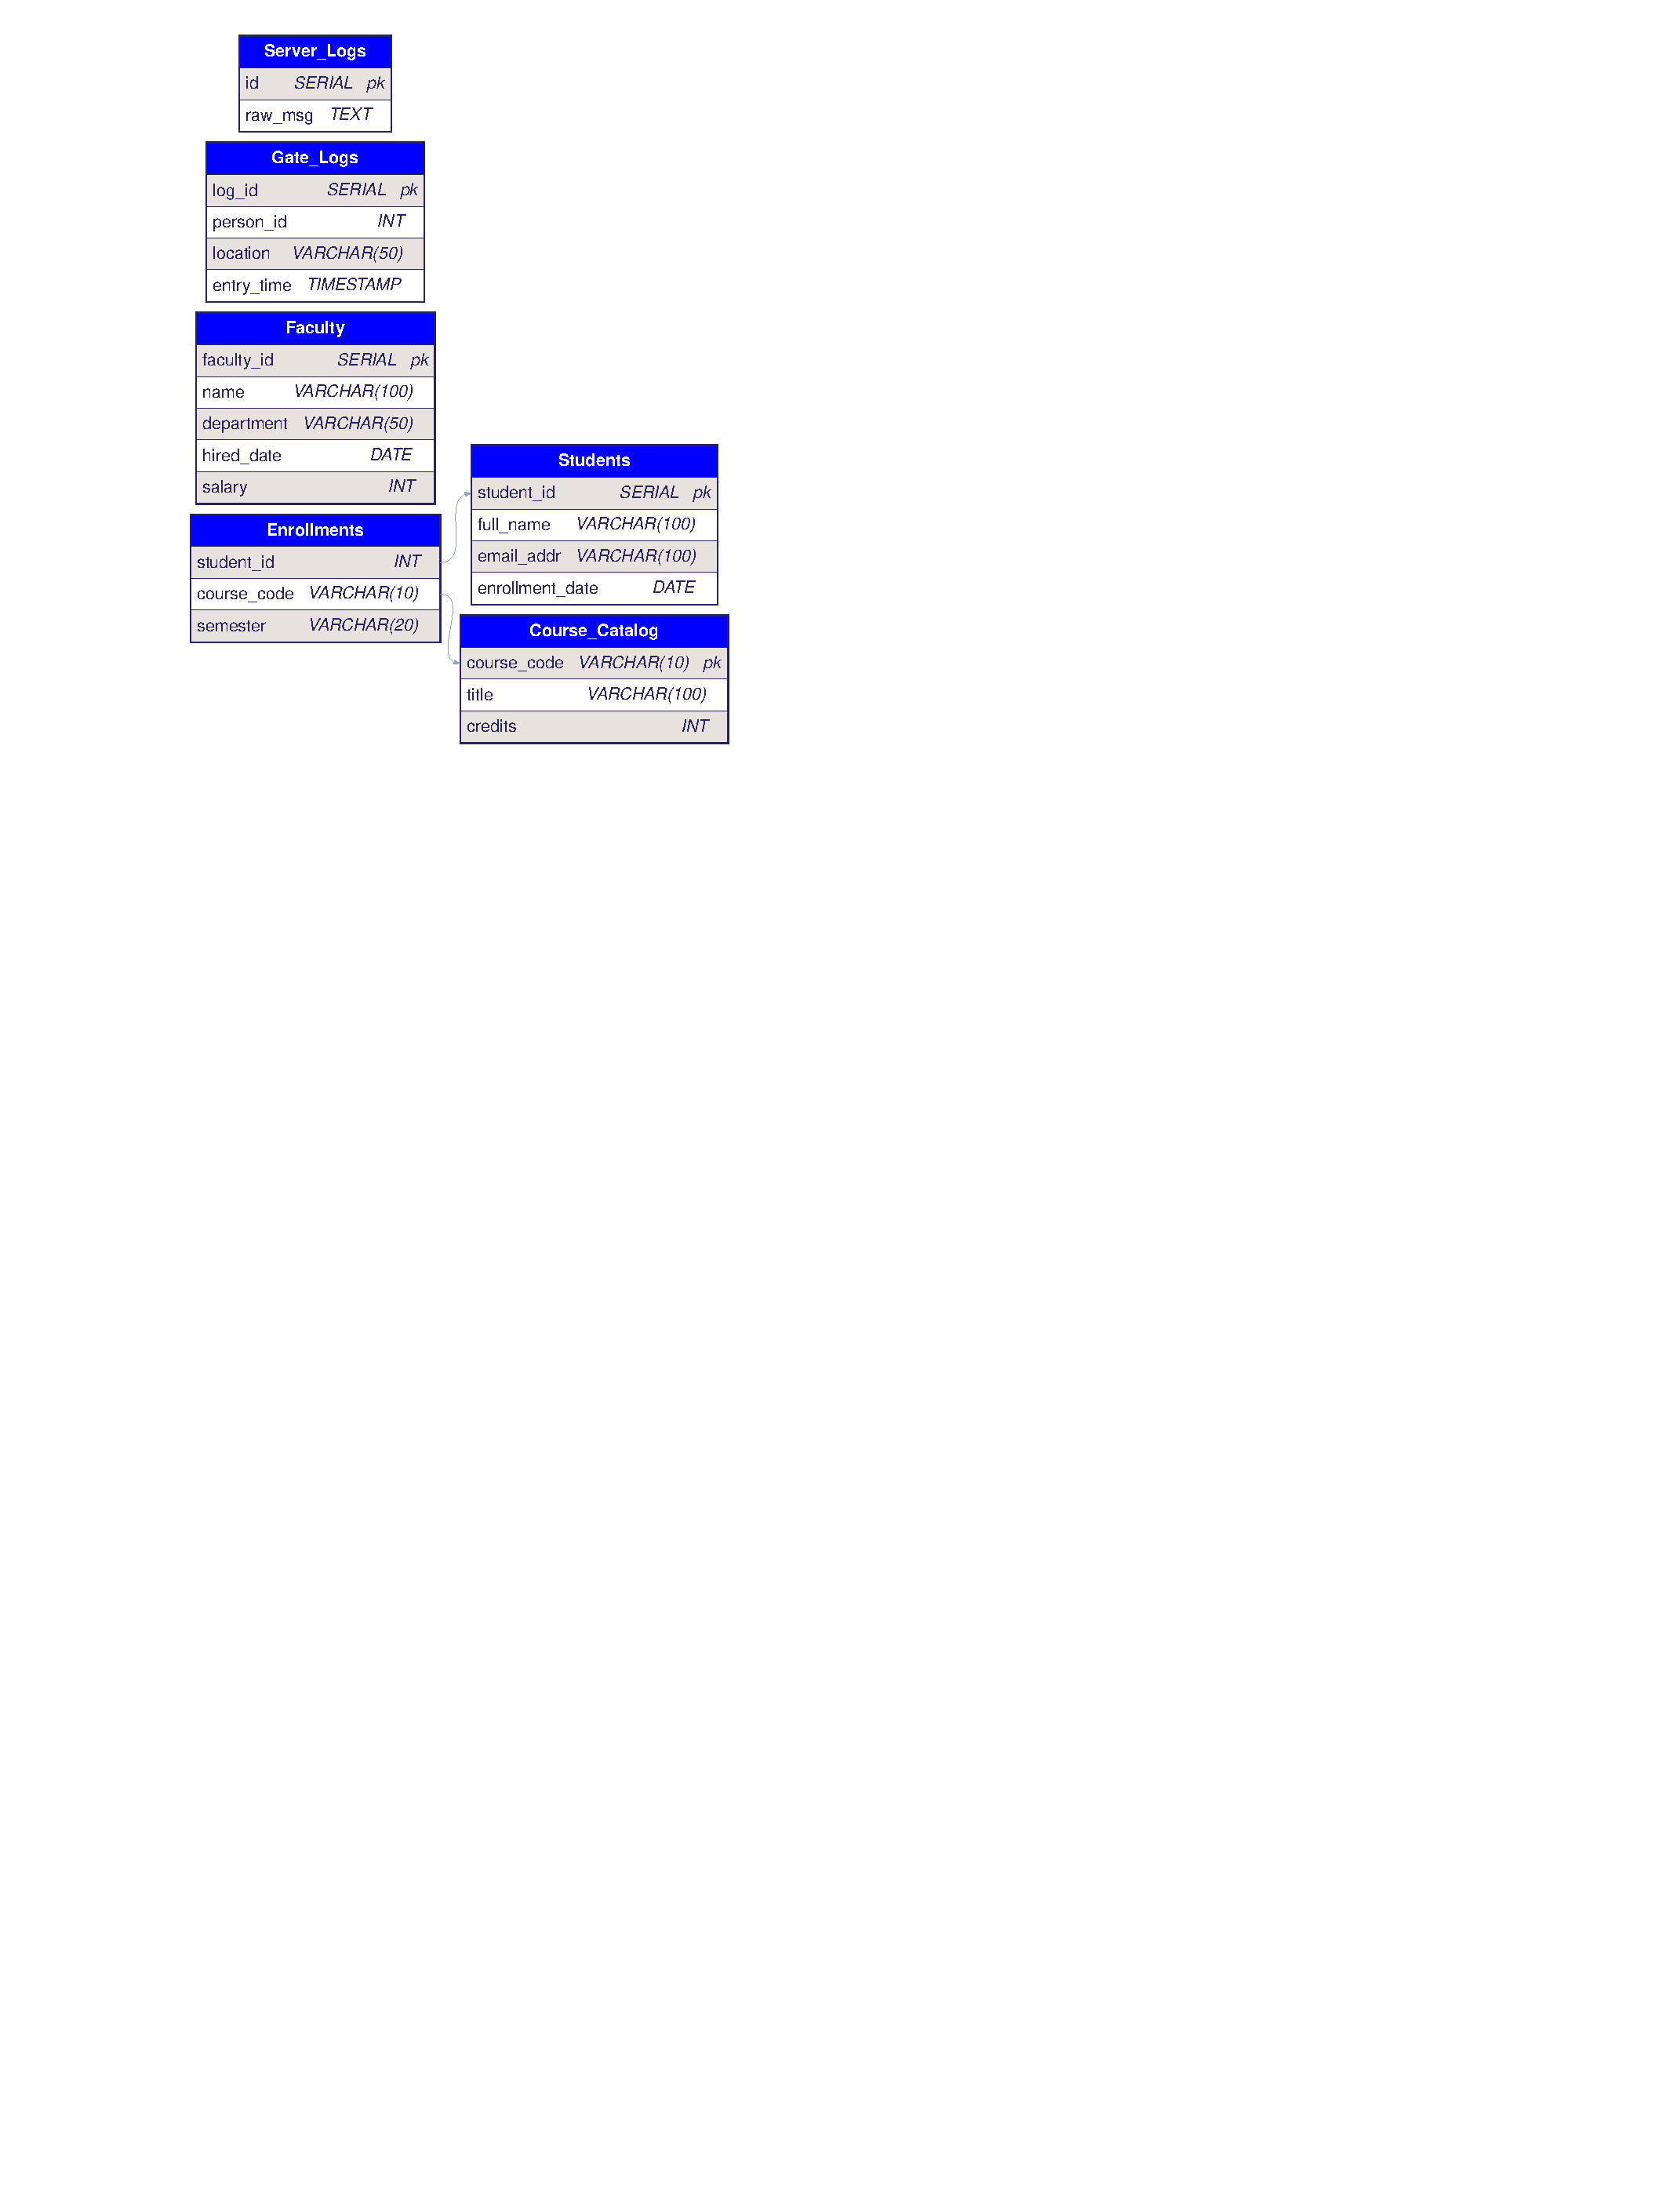
\includegraphics[trim={0cm 31cm 18cm 0cm}, clip, width=0.8\textwidth]{lab_06_erd.pdf}
\end{figure}
% \begin{enumerate}  % all tasks commented out; tasks live in per-section files

% ================================================================== % GROUP 1: STRING MANIPULATION % Topics: INITCAP, UPPER, LOWER, SUBSTR, POSITION, TRIM, REPLACE % ================================================================== \section*{Group 1: Data Normalization (String Functions)}

% \item The student names are currently mixed case (e.g., 'ALICE pendergast'). Write a query to display the \texttt{student\_id} and the \texttt{full\_name} converted to standard Title Case.
% Solution:
% SELECT student_id, INITCAP(full_name) AS clean_name FROM Students;

% \item We need to generate a unique username for each student. Create a query that concatenates the first 3 letters of their name (in lowercase) with their student ID.
% Solution:
% SELECT LOWER(LEFT(full_name, 3)) || student_id AS generated_username FROM Students;

% \item Extract the domain name from the email addresses. You must use \texttt{POSITION} to find the '@' symbol and \texttt{SUBSTR} to get the text after it.
% Solution:
% SELECT email_addr, SUBSTR(email_addr, POSITION('@' IN email_addr) + 1) AS domain FROM Students;

% \item The \texttt{Server\_Logs} table contains entries with leading/trailing whitespace. Display the \texttt{raw\_msg} trimmed of all whitespace.
% Solution:
% SELECT TRIM(raw_msg) FROM Server_Logs;

% \item The system logs use underscores instead of spaces. Use \texttt{REPLACE} to convert \texttt{raw\_msg} content like 'Disk\_Space\_Low' into 'Disk Space Low'.
% Solution:
% SELECT REPLACE(raw_msg, '_', ' ') FROM Server_Logs;

% \item Clean specific characters: Remove the hashtags ('\#') from the beginning and end of the log message '\#\#CRITICAL\_FAILURE\#\#'.
% Solution:
% SELECT TRIM(BOTH '#' FROM raw_msg) FROM Server_Logs WHERE id = 2;
% ================================================================== % GROUP 2: TEMPORAL DATA (Dates \& Times) % Topics: AGE, EXTRACT, CURRENT_DATE % ================================================================== \section*{Group 2: Timeline Analysis (Date Functions)}

% \item Calculate how long each Faculty member has been working at the university. Display their Name and their Tenure (using the \texttt{AGE} function). Assume current date is '2025-01-01'.
% Solution:
% SELECT name, AGE('2026-01-01', hired_date) AS tenure FROM Faculty;

% \item We need to analyze gate traffic by hour. Display the \texttt{location} and the Hour (using \texttt{EXTRACT}) for every entry in \texttt{Gate\_Logs}.
% Solution:
% SELECT location, EXTRACT(HOUR FROM entry_time) AS entry_hour FROM Gate_Logs;

% \item Find the names of students who enrolled in the year 2023. You must use \texttt{EXTRACT(YEAR ...)} in your \texttt{WHERE} clause.
% Solution:
% SELECT full_name FROM Students WHERE EXTRACT(YEAR FROM enrollment_date) = 2023;

% \item Display the Student Name and the number of full years (integer) they have been enrolled. (Hint: \texttt{EXTRACT(YEAR FROM AGE(...))}).
% Solution:
% SELECT full_name, EXTRACT(YEAR FROM AGE(CURRENT_DATE, enrollment_date)) AS years_enrolled FROM Students;

% \item List all gate logs that occurred in the 'PM' (after 12:00). Use \texttt{EXTRACT} to filter by hour.
% Solution:
% SELECT * FROM Gate_Logs WHERE EXTRACT(HOUR FROM entry_time) >= 12;

% \item Calculate the hiring anniversary (Day and Month) for all faculty. Display Name, Hired Month, and Hired Day.
% Solution:
% SELECT name, EXTRACT(MONTH FROM hired_date) as month, EXTRACT(DAY FROM hired_date) as day FROM Faculty;
% ================================================================== % GROUP 3: SET OPERATIONS % Topics: UNION, UNION ALL, INTERSECT, EXCEPT % ================================================================== \section*{Group 3: Set Analysis (Set Operators)}

% \item Create a single list of all unique IDs (Student or Faculty) who have entered EITHER the 'Server Room' OR the 'Chemistry Lab'.
% Solution:
% SELECT person_id FROM Gate_Logs WHERE location = 'Server Room'
% UNION
% SELECT person_id FROM Gate_Logs WHERE location = 'Chemistry Lab';

% \item Identify the "High Risk" individuals: Find the IDs of people who have visited BOTH the 'Server Room' AND the 'Chemistry Lab'.
% Solution:
% SELECT person_id FROM Gate_Logs WHERE location = 'Server Room'
% INTERSECT
% SELECT person_id FROM Gate_Logs WHERE location = 'Chemistry Lab';

% \item Find the Student IDs of those who are taking 'CS102' but are NOT taking 'CS101'.
% Solution:
% SELECT student_id FROM Enrollments WHERE course_code = 'CS102'
% EXCEPT
% SELECT student_id FROM Enrollments WHERE course_code = 'CS101';

% \item Generate a master list of all people associated with the university. Display Name and Role ('Student' or 'Staff') using \texttt{UNION ALL}.
% Solution:
% SELECT full_name as name, 'Student' as role FROM Students
% UNION ALL
% SELECT name, 'Staff' as role FROM Faculty;

% \item Which students (IDs) exist in the system but have NO records in the \texttt{Gate\_Logs}? (Use \texttt{EXCEPT}).
% Solution:
% SELECT student_id FROM Students
% EXCEPT
% SELECT person_id FROM Gate_Logs;

% \item List all unique locations from the logs. Use a Set Operator to ensure distinct values (do not use the DISTINCT keyword).
% Solution:
% SELECT location FROM Gate_Logs UNION SELECT location FROM Gate_Logs;
% ================================================================== % GROUP 4: ADVANCED REPORTING (Joins + Manual Topics) % Topics: JOIN mixed with String/Date functions % ================================================================== \section*{Group 4: Complex Reporting (Joins + Functions)}

% \item Generate a formatted report showing "\texttt{STUDENT\_NAME} enrolled in \texttt{COURSE\_TITLE}". Use \texttt{UPPER} to capitalize the student name.
% Solution:
% SELECT UPPER(s.full_name) as student, c.title
% FROM Students s
% JOIN Enrollments e ON s.student_id = e.student_id
% JOIN Course_Catalog c ON e.course_code = c.course_code;

% \item Find the names of Faculty members who entered the 'Chemistry Lab' in the Morning (before 12:00). You must join \texttt{Faculty} and \texttt{Gate\_Logs} and use \texttt{EXTRACT}.
% Solution:
% SELECT f.name
% FROM Faculty f
% JOIN Gate_Logs g ON f.faculty_id = g.person_id
% WHERE g.location = 'Chemistry Lab' AND EXTRACT(HOUR FROM g.entry_time) < 12;

% \item Display the \texttt{full\_name} of students and the \texttt{domain} of their email, but only for students who have visited the 'Server Room'.
% Solution:
% SELECT s.full_name, SUBSTR(s.email_addr, POSITION('@' IN s.email_addr)+1) as domain
% FROM Students s
% JOIN Gate_Logs g ON s.student_id = g.person_id
% WHERE g.location = 'Server Room';

% \item Count the number of visits to each location, but display the location name in \texttt{UPPER} case.
% Solution:
% SELECT UPPER(location), COUNT(*) 
% FROM Gate_Logs 
% GROUP BY UPPER(location);

% \item Report the average salary of faculty members, grouped by the year they were hired (\texttt{EXTRACT(YEAR...)}).
% Solution:
% SELECT EXTRACT(YEAR FROM hired_date) as hire_year, AVG(salary)
% FROM Faculty
% GROUP BY EXTRACT(YEAR FROM hired_date);

% \item Find students who have been enrolled for more than 2 years. Display Name and Tenure. (Use \texttt{AGE} in the \texttt{WHERE} or \texttt{HAVING} clause).
% Solution:
% SELECT full_name, AGE(CURRENT_DATE, enrollment_date)
% FROM Students
% WHERE EXTRACT(YEAR FROM AGE(CURRENT_DATE, enrollment_date)) > 2;
% ================================================================== % GROUP 5: SECURITY \& DCL % Topics: Views, Materialized Views, WITH CHECK OPTION, GRANT/REVOKE % ================================================================== \section*{Group 5: Access Control (DCL \& Views)}

% \item Create a View named \texttt{View\_Gmail\_Users} that displays only the ID and Name of students who use a '@gmail.com' address.
% Solution:
% CREATE VIEW View_Gmail_Users AS 
% SELECT student_id, full_name FROM Students WHERE email_addr LIKE '%gmail.com';

% \item Create an \textbf{Updatable View} named \texttt{View\_CS\_Courses} that selects all columns from \texttt{Course\_Catalog} where the code starts with 'CS'. Ensure strict data integrity using \texttt{WITH CHECK OPTION}.
% Solution:
% CREATE VIEW View_CS_Courses AS
% SELECT * FROM Course_Catalog WHERE course_code LIKE 'CS%'
% WITH CHECK OPTION;

% \item Create a \textbf{Materialized View} named \texttt{MatView\_Enrollment\_Stats} that counts how many students are in each course.
% Solution:
% CREATE MATERIALIZED VIEW MatView_Enrollment_Stats AS
% SELECT course_code, COUNT(*) as total FROM Enrollments GROUP BY course_code;

% \item Write the command to refresh the data in \texttt{MatView\_Enrollment\_Stats}.
% Solution:
% REFRESH MATERIALIZED VIEW MatView_Enrollment_Stats;

% \item Create a Group Role named \texttt{research\_assistants} (cannot login), then create a user \texttt{bob} and add him to this group.
% Solution:
% CREATE ROLE research_assistants NOLOGIN;
% CREATE ROLE bob LOGIN PASSWORD 'pass';
% GRANT research_assistants TO bob;

% \item Grant the \texttt{research\_assistants} group permission to SELECT from the \texttt{Students} table, but only the \texttt{full\_name} and \texttt{email\_addr} columns (hiding the enrollment date).
% Solution:
% GRANT SELECT (full_name, email_addr) ON Students TO research_assistants;
% \end{enumerate}
\end{document}